\documentclass[10pt,twocolumn]{article}
\usepackage[a4paper,margin=1.8cm,columnsep=0.6cm]{geometry}
\usepackage[T1]{fontenc}
\usepackage{lmodern,microtype}
\usepackage{amsmath,amssymb,bm}
\usepackage{graphicx,booktabs,multirow,array,xcolor,colortbl}
\usepackage[numbers,sort&compress]{natbib}
\usepackage[hidelinks]{hyperref}
\usepackage{tikz}
\usetikzlibrary{arrows.meta,positioning,fit,calc}
\usepackage{caption}
\captionsetup{font=small,labelfont=bf}
\usepackage{enumitem}
\setlist{nosep,leftmargin=*}

\newcommand{\best}[1]{\textbf{#1}}
\newcommand{\worst}[1]{\textcolor{red!70!black}{#1}}
\definecolor{keybg}{RGB}{238,244,250}

\title{\vspace{-1.2em}\textbf{Does the Uncertainty Notice? A Comparative Study of Variational JEPA Experts and Fusion Rules for Multimodal Sentiment Analysis under Missing and Corrupted Modalities}}
\author{Final Year Project, Part I \\ \small Code and data: \url{https://github.com/fasihh/bigthing} (folder \texttt{JF/})}
\date{\small November 2026}

\begin{document}
\maketitle

\begin{abstract}
A multimodal model should not only be accurate when every input is present: when an input is missing, corrupted or
contradicts the others, its stated uncertainty should grow and its prediction ranges should stay honest. We study this
on CMU-MOSEI sentiment regression with one probabilistic \emph{expert} per modality (text, audio, video), each
outputting a Gaussian belief over a shared latent. We compare four ways of pretraining the experts without labels
(variational JEPA, reconstruction, contrastive alignment, none), three training regimes (frozen, fine-tuned,
supervised) and four fusion rules (product of experts, prior-corrected product, mixture of experts, attention),
over 46 test conditions and three seeds (144 trained models). We add a multimodal \emph{noisy TV}: noise added at test
time, a pure-noise extra modality, swapped modalities and a sticky distractor injected into every modality, and we
reproduce the original variational JEPA noisy TV experiment with 15 seeds.
\textbf{Findings.} (i)~Product of experts is the most accurate fusion in every regime (fine-tuned MAE 0.56, NLL 1.26)
and MoE the least (MAE 0.64, NLL 1.31). (ii)~When an input is \emph{declared} missing, uncertainty tracks the error
(tracking ratio 0.96--1.04, ideal 1.0). (iii)~When an input is \emph{silently} corrupted, it does not: replacing the
text with pure noise raises the error by 17--55\% while the text expert's $\sigma$ stays flat or falls, coverage of
90\% ranges drops to 0.75--0.80, and $\sigma$ detects swapped modalities at chance (AUROC 0.50). (iv)~A shared sticky
distractor hijacks every self-supervised objective (sentiment probe $R^2$ 0.33$\rightarrow$0.07); only supervised
training resists it. (v)~The original variational JEPA results reproduce exactly, but on 10 new seeds a deterministic
JEPA beats the variational one in 7/10 seeds, and one seed makes the variational model fail ($R^2=-6.4$). Learned
Gaussian uncertainty is therefore \emph{aleatoric only}: it sees noise in the data, not a broken sensor.
(vi)~A final run (159 stage-2 models, S-JEPA, MoNIG and concatenation added) reproduces these numbers, and ablations of candidate
fixes show what does help: a variational \emph{target} lifts corruption detection by $\sigma$ from below chance
(AUROC 0.38) to 0.71; cross-examining the experts against each other localises a corrupted sensor on a second dataset
(MS-COCO, AUROC 0.75--0.95, MAE 0.570$\rightarrow$0.524); and a screen of 30 techniques shows that input-level detectors
flag held-out corruptions (AUROC 0.82 on MOSEI) where $\sigma$ cannot. These results motivate Part~II.
\end{abstract}

% ------------------------------------------------------------------------------------------------
\section{Introduction}
Multimodal systems are deployed where sensors fail. A camera is covered, a microphone picks up a television, a
transcript belongs to another speaker. A useful system must then do two things: keep its point prediction as good
as the remaining inputs allow, and \emph{say} that it is less sure. The second requirement is rarely measured.
Accuracy tables on clean benchmarks dominate the multimodal sentiment literature~\cite{zadeh2018mosei,mao2022msena}.

Joint-embedding predictive architectures (JEPA)~\cite{lecun2022path,assran2023ijepa} learn representations by
predicting the latent of one view from another, rather than reconstructing inputs. Variational JEPA~\cite{huang2026vjepa}
makes the predictor output a distribution, and BJEPA fuses it with prior experts by a Product of Experts (PoE). The
original work argues that predicting in latent space ignores unpredictable nuisance (the ``noisy TV''~\cite{burda2019curiosity}).
Multimodal fusion maps naturally onto this: each modality becomes a probabilistic expert, and a PoE gives more weight
to the more confident one, which is the behaviour we want when a modality is missing.

This report is a \emph{comparative study}. We ask, with numbers rather than anecdotes:
\begin{enumerate}
  \item Which fusion rule is most accurate and best calibrated when modalities are missing?
  \item Does the predicted uncertainty rise as much as the error does, when an input is missing and when it is corrupted?
  \item Does the pretraining objective (variational JEPA vs.\ reconstruction vs.\ contrastive alignment) matter?
  \item Does a variational JEPA ignore a noise source in the multimodal case, as it is claimed to in the single-stream case?
  \item Do the published noisy TV results hold on new random seeds?
  \item How much do calibrated prediction ranges (post-hoc scaling, conformal prediction) fix?
\end{enumerate}

\paragraph{Contributions.}
(1)~A controlled benchmark of 144 models (72 for the main comparison of objectives, regimes and fusion rules, and 72 trained
with a noise source), each over 3 seeds, evaluated on 46 test conditions with 7 decoders and more than 40 metrics.
(2)~A \emph{multimodal noisy TV} protocol with four variants (test-time noise, noise modality, swapped
modality, sticky distractor).
(3)~A \emph{tracking ratio} that measures whether uncertainty rises in proportion to the error.
(4)~A 15-seed reproduction of the variational JEPA noisy TV experiment.
(5)~The finding that learned Gaussian uncertainty misses silent corruption: it is calibrated for missing
inputs but blind to broken ones.

% ------------------------------------------------------------------------------------------------
\section{Background and related work}
\paragraph{JEPA and its probabilistic variants.} I-JEPA~\cite{assran2023ijepa} predicts target-encoder latents of masked
regions from a context encoder; the target encoder is an exponential moving average (EMA) of the context encoder, as in
BYOL~\cite{grill2020byol}. Variational JEPA (VJEPA)~\cite{huang2026vjepa} replaces the point predictor with a Gaussian one
and trains it by likelihood. BJEPA combines VJEPA with prior experts through a PoE. Var-JEPA~\cite{gogl2026varjepa}
derives JEPA from an evidence lower bound. S-JEPA~\cite{giakoumoglou2026sjepa} adds a stochastic latent with a learned
prior. All of them model \emph{aleatoric} uncertainty: how unpredictable the target is from the context.

\paragraph{Multimodal fusion with uncertainty.} The MVAE~\cite{wu2018mvae} fuses modality posteriors by a PoE with a
standard-normal prior expert, and MMVAE~\cite{shi2019mmvae} uses a mixture (MoE). Evidential approaches place
Dirichlet~\cite{han2021tmc} or Normal-Inverse-Gamma~\cite{ma2021monig,amini2020evidential} beliefs on each view. MoNIG
was evaluated on CMU-MOSEI.

\paragraph{Calibration and conformal prediction.} Post-hoc temperature scaling~\cite{guo2017calibration} rescales
predicted variance. Split conformal prediction~\cite{vovk2005algorithmic,angelopoulos2021gentle} gives distribution-free
coverage under exchangeability. Under missing modalities, a single pooled quantile over-covers some
modality patterns and under-covers others, which motivates per-pattern (Mondrian) calibration~\cite{mccf2026}. We
score probabilistic predictions with proper scores (NLL, CRPS)~\cite{gneiting2007scoring} and selective
prediction~\cite{geifman2017selective}.

% ------------------------------------------------------------------------------------------------
\section{Method}
\begin{figure}[t]
\centering
\resizebox{\columnwidth}{!}{%
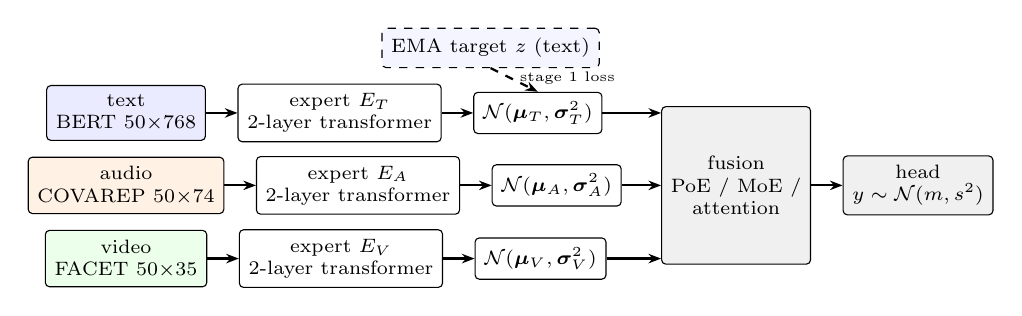
\begin{tikzpicture}[font=\scriptsize, node distance=3mm,
  box/.style={draw, rounded corners=1.5pt, minimum height=5mm, align=center, fill=white},
  arr/.style={-{Stealth[length=1.6mm]}, thick}]
\node[box, fill=blue!8] (t) {text\\BERT 50$\times$768};
\node[box, fill=orange!10, below=2mm of t] (a) {audio\\COVAREP 50$\times$74};
\node[box, fill=green!8, below=2mm of a] (v) {video\\FACET 50$\times$35};
\foreach \m/\n in {t/T, a/A, v/V}{
  \node[box, right=4mm of \m] (e\m) {expert $E_{\n}$\\2-layer transformer};
  \node[box, right=4mm of e\m] (b\m) {$\mathcal{N}(\bm\mu_{\n},\bm\sigma_{\n}^2)$};
  \draw[arr] (\m) -- (e\m); \draw[arr] (e\m) -- (b\m);}
\node[box, fill=gray!12, right=5mm of ba, minimum height=20mm] (f) {fusion\\PoE / MoE /\\attention};
\foreach \m in {t,a,v} \draw[arr] (b\m.east) -- (f.west |- b\m.east);
\node[box, right=4mm of f, fill=gray!12] (h) {head\\$y\sim\mathcal{N}(m,s^2)$};
\draw[arr] (f) -- (h);
\node[box, dashed, above=3mm of bt, xshift=-6mm, fill=blue!4] (tg) {EMA target $z$ (text)};
\draw[arr, dashed] (tg.south) -- node[right, pos=.4]{\tiny stage 1 loss} (bt.north);
\end{tikzpicture}}
\caption{Architecture. Stage 1 (no labels) trains each expert to predict a target latent (here: the EMA text latent
for variational JEPA). Stage 2 (labels) trains the fusion and head. Missing modalities are simply left out of the fusion.}
\label{fig:arch}
\end{figure}

\paragraph{Experts.} Each modality $m\in\{T,A,V\}$ has an expert $E_m$: a linear input projection, learned positional
embeddings, a 2-layer pre-norm transformer (width 128, 4 heads), masked mean pooling, and a predictor that outputs a
diagonal Gaussian belief $\mathcal{N}(\bm\mu_m,\mathrm{diag}\,\bm\sigma_m^2)$ over a 64-dimensional latent, with
$\log\sigma^2$ bounded to $[-6,4]$.

\paragraph{Stage 1: label-free pretraining.} We compare four objectives.
\emph{Variational JEPA (V-JEPA)}: an EMA copy of the text encoder produces a layer-normalised target $\bm z$; every
expert sees its input with 40\% of time steps masked and maximises the likelihood of $\bm z$:
\begin{multline}
\mathcal{L} = \sum_{m}\Big[-\log\mathcal{N}(\bm z;\bm\mu_m,\bm\sigma_m^2) + \beta\,\mathrm{KL}_m\Big]\\
 - \log\mathcal{N}\big(\bm z;\mathrm{PoE}_{S}\big) + \mathcal{L}_{\mathrm{VIC}},
\end{multline}
where $\mathrm{PoE}_S$ fuses a random subset $S$ of experts, $\beta=10^{-3}$, and VICReg~\cite{bardes2022vicreg} on the
online text encoder prevents collapse. \emph{Reconstruction}: an MVAE~\cite{wu2018mvae} that decodes every modality's
time-averaged features from PoE-fused samples of several subsets. \emph{Alignment}: InfoNCE~\cite{oord2018cpc} between
each expert's mean and the text latent, with a variance head fitted afterwards. \emph{None}: no pretraining.

\paragraph{Fusion.} Given the available experts, \textbf{PoE} multiplies the Gaussians together with an $\mathcal{N}(\bm 0,\bm I)$ prior:
$\bm P=\bm 1+\sum_m\bm\sigma_m^{-2}$, $\bm\mu=\bm P^{-1}\sum_m\bm\sigma_m^{-2}\bm\mu_m$. \textbf{Prior-corrected PoE} removes
the $n-1$ duplicated priors. \textbf{MoE} moment-matches a uniform mixture of the available experts, and \textbf{attention} learns the
mixture weights.

\paragraph{Stage 2: head.} A linear head maps the fused belief to the label while propagating its variance,
$y\sim\mathcal{N}\big(\bm w^\top\bm\mu+b,\ \alpha\sum_i w_i^2\sigma_i^2+s^2\big)$, and is trained by Gaussian NLL. Every
training clip gets a random non-empty subset of modalities. Experts are either \emph{frozen}, \emph{fine-tuned}, or
trained from scratch (\emph{supervised}).

\paragraph{Decoders.} Prediction ranges at level $p$ are produced by: D0, a point decoder trained with squared error,
$\pm$ a constant width; D1, the head mean $\pm$ a constant width; D2, the raw Gaussian, $\pm z_p\sigma$; D3a, post-hoc
rescaling, $\pm z_p\tau\sigma$; D3b, normalised split conformal, $\pm q_p\sigma$; and D3c, conformal calibrated per test
condition (an oracle reference). All calibration uses the validation split, pooled over all conditions.

% ------------------------------------------------------------------------------------------------
\section{Experimental setup}
\paragraph{Data.} CMU-MOSEI~\cite{zadeh2018mosei} in the MMSA release~\cite{mao2022msena} (\texttt{aligned\_50.pkl}):
16,326 / 1,871 / 4,659 clips for train / validation / test. The single label is the sentiment score in $[-3,3]$. Text features are
BERT~\cite{devlin2019bert} token embeddings (PCA to 128 dimensions fitted on train, keeping 67.0\% of the variance), audio is COVAREP~\cite{degottex2014covarep}
(74-d) and video is FACET (35-d). Audio and video are standardised with training statistics.

\paragraph{Test conditions (46).} \emph{Missing}: all 7 non-empty modality subsets. \emph{Partly missing text}: 25--90\% of
text tokens hidden. \emph{Noisy TV A}: $x'=\sqrt{1-\lambda}\,x+\sqrt{\lambda}\,\varepsilon$ on any combination of
modalities, $\lambda\in\{.25,.5,.75,1\}$, with $\varepsilon$ matched to each feature's spread. The corrupted input is still
presented as available. \emph{Noisy TV C}: audio and/or video swapped in from another clip.
Two further grids are trained with the corruption present. \emph{Noisy TV B} adds a fourth, pure-noise modality.
\emph{Noisy TV D} adds a sticky distractor $d_t=0.9\,d_{t-1}+\sqrt{0.19}\,\eta_t$ (8-d), mixed into every modality's features
at $\sigma=2$ or $8$ times the feature spread, either independent per modality or shared. This follows the original noisy
TV design~\cite{huang2026vjepa}.

\paragraph{Metrics.} Accuracy: MAE, binary accuracy (Acc2). Probabilistic: NLL, CRPS, calibration error, coverage of
90\% ranges (Cov90), interval width. Uncertainty quality: Spearman rank correlation of $\sigma$ with $|$error$|$, AUROC
for flagging errors $>1$, excess area under the risk--coverage curve. We also define the \textbf{tracking ratio}:
\begin{equation}
\mathrm{TR}=\frac{\overline{\sigma}_{\text{without text}}\,/\,\overline{\sigma}_{\text{with text}}}{\mathrm{MAE}_{\text{without text}}\,/\,\mathrm{MAE}_{\text{with text}}},
\end{equation}
which is 1 when $\sigma$ rises exactly as much as the error, and below 1 when the model becomes overconfident. Probes:
ridge regression from the fused latent to the sentiment (signal $R^2$) and to the distractor (distractor $R^2$).

\paragraph{Protocol.} Three seeds (0, 1, 2). Stage 1: 30 epochs, AdamW, learning rate $3\!\times\!10^{-4}$, cosine schedule.
Stage 2: up to 40 epochs with early stopping on the mean validation NLL over the 7 subsets. All corruptions use fixed
seeds, so every model sees identical inputs. Totals: 72 main, 48 distractor and 24 noise-modality models, about 5 GPU-hours.
Values are mean $\pm$ standard deviation over seeds. A \emph{final run} (Section~\ref{sec:final}) repeats the study with the
EMA-dropout issue fixed, adds S-JEPA~\cite{giakoumoglou2026sjepa}, MoNIG~\cite{ma2021monig}, concatenation and late averaging,
and trains 159 stage-2 models; frozen PoE reproduces to within 0.002 NLL (1.420 vs.\ 1.422) and 0.000 Cov90 (0.892).

% ------------------------------------------------------------------------------------------------
\section{Results}
\begin{table}[t]
\centering\small
\colorbox{keybg}{\parbox{0.96\columnwidth}{\centering
\textbf{Key numbers}\\[2pt]
\resizebox{0.94\columnwidth}{!}{\begin{tabular}{@{}l r@{}}
Best MAE (all modalities), PoE fine-tuned & \textbf{0.558--0.564}\\
MoE MAE in the same setting & 0.637--0.650\\
Tracking ratio, text declared missing (frozen PoE) & \textbf{1.007} (ideal 1)\\
Tracking ratio, text silently replaced by noise & 0.63--0.86\\
Cov90 when text is pure noise (fine-tuned, raw) & \worst{0.789} (target 0.90)\\
Swap detection AUROC by $\sigma$ (all models) & \worst{0.49--0.55}\\
Swap detection AUROC by disagreement (frozen) & 0.56--0.87\\
Signal $R^2$, V-JEPA, shared distractor & \worst{0.33 $\to$ 0.07}\\
Huang reproduction, max.\ difference & 0.000\\
JEPA beats VJEPA (new seeds) & 7/10\\
\midrule
\multicolumn{2}{@{}l}{\emph{Final run and ablations (Sec.~\ref{sec:final})}}\\
$\sigma$ ratio / MAE ratio, text = noise (all fusions) & \worst{1.00} / 1.16\\
Corruption AUROC by $\sigma$: V-JEPA $\to$ variational target & \worst{0.38} $\to$ \best{0.71}\\
COCO, one sensor corrupted, MAE: PoE $\to$ CXF & 0.570 $\to$ \best{0.524}\\
MOSEI, replaced-input detector, held-out AUROC & \best{0.82}
\end{tabular}}}}
\end{table}

\subsection{Accuracy and calibration with missing modalities}
\begin{table*}[t]
\centering\small
\caption{Accuracy and calibration on CMU-MOSEI (test). MAE and Acc2 use all modalities (TAV); ``no text'' = audio+video only. NLL,
calibration error (CalErr) and Cov90 are averaged over the 7 modality subsets, using the raw Gaussian (D2). Mean $\pm$ std over 3 seeds. Best per column in bold.}
\label{tab:main}
\setlength{\tabcolsep}{4pt}
\begin{tabular}{llllllll}
\toprule
Objective & Regime & Fusion & MAE TAV $\downarrow$ & MAE no text $\downarrow$ & Acc2 TAV $\uparrow$ & NLL $\downarrow$ & Cov90 (0.90)\\
\midrule
\multirow{4}{*}{V-JEPA} & frozen & PoE & 0.727$\pm$.019 & 0.817$\pm$.002 & 0.766$\pm$.022 & 1.420$\pm$.018 & 0.892$\pm$.003\\
 & frozen & MoE & 0.756$\pm$.012 & 0.816$\pm$.002 & 0.745$\pm$.021 & 1.441$\pm$.014 & 0.889$\pm$.001\\
 & fine-tuned & PoE & 0.563$\pm$.006 & 0.809$\pm$.006 & 0.843$\pm$.005 & 1.261$\pm$.004 & 0.883$\pm$.006\\
 & fine-tuned & MoE & 0.641$\pm$.002 & \best{0.798}$\pm$.001 & 0.820$\pm$.008 & 1.311$\pm$.003 & 0.881$\pm$.008\\
 & fine-tuned & attention & 0.564$\pm$.007 & 0.810$\pm$.003 & 0.845$\pm$.004 & 1.264$\pm$.004 & 0.874$\pm$.010\\
\midrule
Recon. & frozen & PoE & 0.713$\pm$.007 & 0.813$\pm$.005 & 0.778$\pm$.009 & 1.403$\pm$.004 & \best{0.893}$\pm$.000\\
Recon. & fine-tuned & PoE & 0.564$\pm$.005 & 0.811$\pm$.003 & \best{0.847}$\pm$.004 & 1.268$\pm$.005 & 0.878$\pm$.004\\
Align. & frozen & PoE & 0.701$\pm$.008 & 0.816$\pm$.001 & 0.776$\pm$.006 & 1.391$\pm$.008 & 0.889$\pm$.000\\
Align. & fine-tuned & PoE & 0.564$\pm$.003 & 0.816$\pm$.005 & 0.843$\pm$.004 & 1.272$\pm$.002 & 0.869$\pm$.006\\
None & supervised & PoE & \best{0.558}$\pm$.005 & 0.813$\pm$.007 & \best{0.847}$\pm$.006 & 1.258$\pm$.005 & 0.872$\pm$.005\\
None & supervised & MoE & 0.637$\pm$.005 & 0.800$\pm$.002 & 0.825$\pm$.002 & 1.314$\pm$.009 & 0.882$\pm$.009\\
None & supervised & attention & 0.565$\pm$.013 & 0.810$\pm$.010 & 0.844$\pm$.007 & \best{1.256}$\pm$.011 & 0.888$\pm$.007\\
\bottomrule
\end{tabular}
\end{table*}

Table~\ref{tab:main} gives the main comparison. \textbf{PoE and attention beat MoE in every regime}: fine-tuned
MAE 0.563 vs.\ 0.641 and NLL 1.261 vs.\ 1.311 with V-JEPA experts, and the same ordering holds for every objective.
MoE averages a strong text belief with weak audio and video beliefs, which dilutes the prediction. PoE lets the
most confident expert dominate. MoE is slightly better only when text is absent (0.798 vs.\ 0.809).

\textbf{Fine-tuning decides accuracy; the objective does not.} Fine-tuned experts from any objective reach MAE
0.563--0.564, and experts trained from scratch reach 0.558. The pretraining objective matters only when experts
are frozen, where alignment (0.701) and reconstruction (0.713) are better than V-JEPA (0.727). With 16k labelled clips,
label-free pretraining on the same clips adds no accuracy.

\textbf{Raw calibration is reasonable on average} (Cov90 0.87--0.89, calibration error 0.02--0.04), but it hides
the subset where it fails. Figure~\ref{fig:cov} breaks coverage down by condition. Fine-tuned PoE covers only 0.862 of
clips when text is missing and 0.789 when text is pure noise. Constant-width ranges (D1) are worse: 0.79 when
text is missing. Split conformal (D3b) repairs the declared-missing case (0.886) but not silent corruption (0.813).

\begin{figure}[t]
\centering
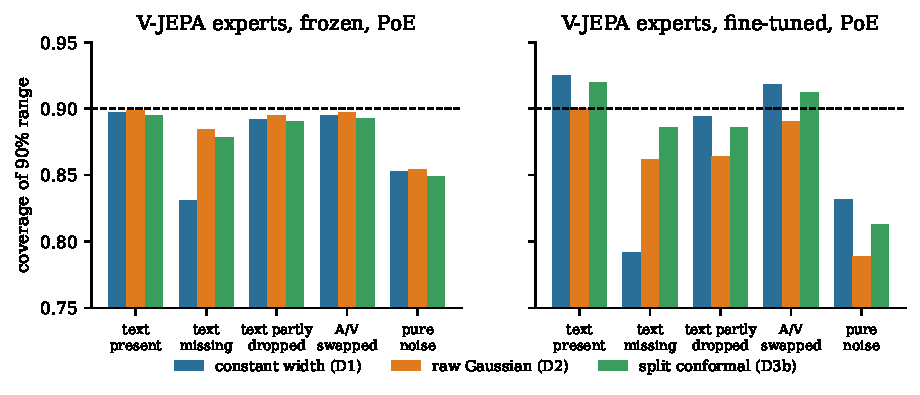
\includegraphics[width=\columnwidth]{figures/coverage_by_condition.pdf}
\caption{Coverage of 90\% prediction ranges by condition (V-JEPA experts, PoE). Dashed: target. No decoder reaches 0.90 when
the text is pure noise. Conformal calibration (green) fixes declared missing text but not silent corruption.}
\label{fig:cov}
\end{figure}

\subsection{Does $\sigma$ track the error?}
\begin{figure}[t]
\centering
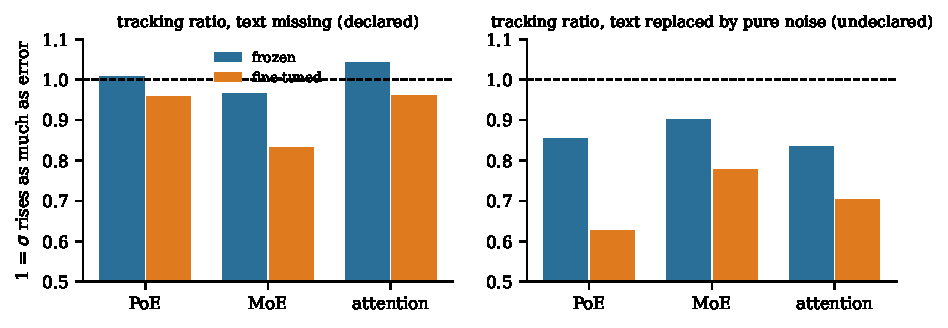
\includegraphics[width=\columnwidth]{figures/tracking.pdf}
\caption{Tracking ratio (1 = $\sigma$ rises exactly as much as the error). Left: text declared missing. Right: text
replaced by pure noise but still presented as available. Every fusion rule under-reacts to silent corruption, and fine-tuning makes it worse.}
\label{fig:track}
\end{figure}

When text is \emph{declared} missing, $\sigma$ tracks the error almost perfectly: the tracking ratio is 1.007 for
frozen V-JEPA with PoE and 0.96 fine-tuned (Fig.~\ref{fig:track}, left). PoE gets this for free: removing the text
expert removes its precision. When text is \emph{silently} replaced by noise, the tracking ratio falls to 0.86 (frozen)
and 0.63 (fine-tuned). The model becomes more confident than it should be, exactly when it is most wrong.

\begin{figure}[t]
\centering
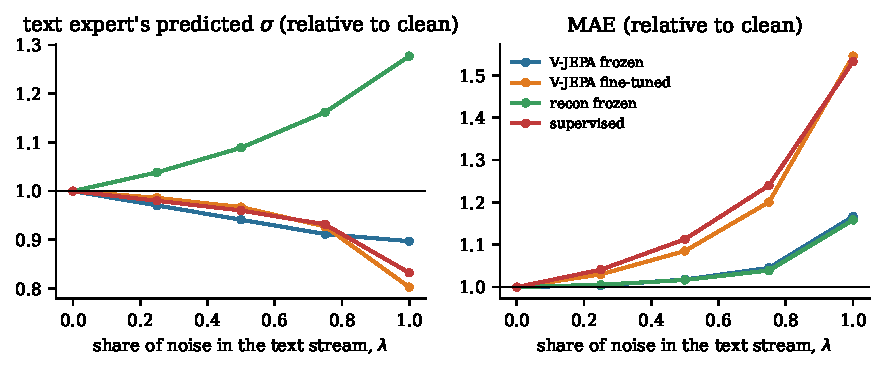
\includegraphics[width=\columnwidth]{figures/noisytv_text.pdf}
\caption{Noisy TV A on the text stream (PoE). Left: the text expert's predicted $\sigma$. Right: the error. The error grows
up to 55\% while $\sigma$ stays flat or \emph{falls}. Only reconstruction experts raise $\sigma$ (by 28\%), and they still under-react.}
\label{fig:noise}
\end{figure}

Figure~\ref{fig:noise} shows the mechanism. As $\lambda$ goes from 0 to 1, the V-JEPA text expert's $\sigma$ \emph{falls}
from 0.068 to 0.061, and its share of the PoE precision stays at 0.89, while the error rises from 0.727 to 0.848. A
Gaussian predictor head trained on clean data maps unfamiliar input to a familiar-looking, confident belief. It
estimates \emph{aleatoric} noise, not \emph{epistemic} doubt~\cite{kendall2017uncertainties}.

\begin{table}[t]
\centering\small
\caption{Swapped modality (Noisy TV C, A and V swapped together): can the system flag the clip? AUROC (0.5 = chance) and Cov90 with D3b.}
\label{tab:swap}
\setlength{\tabcolsep}{3pt}
\resizebox{\columnwidth}{!}{\begin{tabular}{lllll}
\toprule
Objective / regime & Fusion & by $\sigma$ & by disagreement & Cov90\\
\midrule
V-JEPA frozen & PoE & \worst{0.510} & 0.586 & 0.892\\
V-JEPA frozen & MoE & 0.545 & 0.586 & 0.885\\
Align.\ frozen & PoE & \worst{0.491} & \best{0.868} & 0.881\\
Align.\ frozen & MoE & 0.752 & \best{0.868} & 0.870\\
V-JEPA fine-tuned & PoE & \worst{0.500} & 0.502 & 0.906\\
Supervised & PoE & \worst{0.498} & 0.504 & 0.904\\
\bottomrule
\end{tabular}}
\end{table}

Swapping audio and video in from another clip (Table~\ref{tab:swap}) is invisible to $\sigma$: AUROC 0.49--0.51 for
PoE. The \emph{disagreement} between experts (mean symmetric KL) does carry the signal when experts are frozen:
0.87 for alignment experts, which were trained to agree, and 0.59 for V-JEPA. \textbf{Fine-tuning erases it} (0.50).
The cross-modal structure learned in stage 1 is the only label-free cue for conflict, and stage 2 destroys it.

\subsection{Failure detection and selective prediction}
For fine-tuned and supervised models, $\sigma$ ranks errors moderately (Spearman 0.20--0.23, AUROC for errors above
1 point 0.65), and the MAE of the 80\% most confident clips is 0.58--0.60. For frozen V-JEPA experts (any fusion rule),
$\sigma$ is uninformative (Spearman $-0.01$ to $0.06$, AUROC 0.48--0.55). The frozen V-JEPA latent is well calibrated
\emph{as a prediction of the target} (Mahalanobis$^2/d=0.98$, latent Cov90 0.97 with all modalities), but that
uncertainty is about the target, not about the sentiment.

\subsection{Multimodal noisy TV: a noise modality and a sticky distractor}
\begin{table}[t]
\centering\small
\caption{Noisy TV B (final run): a fourth, pure-noise modality is present in training and test. Weight = its share of the
fused prediction (0 is ideal; 0.25 = treated like a real modality). Frozen experts, mean over 3 seeds.}
\label{tab:noisech}
\setlength{\tabcolsep}{4pt}
\begin{tabular}{lcccc}
\toprule
Objective & PoE & attention & MoNIG & MoE / concat\\
\midrule
V-JEPA & 0.045 & \best{0.018} & 0.102 & \worst{0.250}\\
S-JEPA & \best{0.034} & 0.031 & 0.141 & \worst{0.250}\\
Recon. & \worst{0.314} & 0.022 & 0.099 & \worst{0.250}\\
Align. & 0.067 & 0.027 & 0.080 & \worst{0.250}\\
\bottomrule
\end{tabular}
\end{table}

A pure-noise modality (Table~\ref{tab:noisech}) is ignored by attention under every objective (weight 0.02--0.03). PoE
ignores it only when the experts are self-predictive (JEPA, S-JEPA: 0.03--0.05); with reconstruction experts the noise
expert keeps 31\% of the weight, because reconstructing noise yields a confident-looking belief. MoE and concatenation
cannot discount it at all. (The first run, with dropout left on in the EMA target, gave PoE weights of 0.13--0.38;
fixing it mainly helped the JEPA objectives.) Accuracy is barely affected, because the noise belief sits near the prior mean.

\begin{figure}[t]
\centering
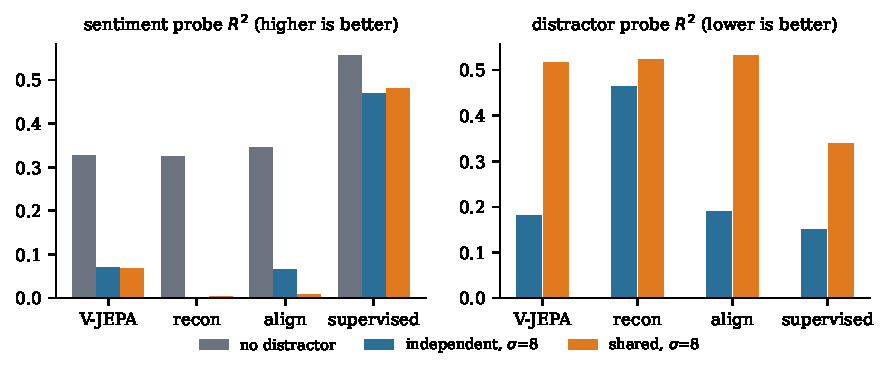
\includegraphics[width=\columnwidth]{figures/distractor_probes.pdf}
\caption{Noisy TV D at $\sigma=8$: how much sentiment and distractor a linear probe recovers from the fused latent. Every
self-supervised objective loses the sentiment; a distractor shared across modalities is absorbed (distractor $R^2\approx0.52$).}
\label{fig:dist}
\end{figure}

The sticky distractor (Fig.~\ref{fig:dist}) is the most damaging condition. At $\sigma=8$, every self-supervised
objective loses the sentiment: signal $R^2$ falls from 0.33 to 0.07 (V-JEPA), 0.00 (reconstruction) and 0.01--0.07
(alignment). When the same distractor appears in all modalities, the latent encodes it (distractor $R^2$ 0.52--0.53).
The reason is structural. The V-JEPA target is computed from the text, which contains the distractor, and the distractor is the most predictable
thing in every stream. A self-predictive objective is \emph{designed} to keep predictable content. Supervised experts keep
the sentiment (0.47--0.48), because labels tell them what matters. So the single-stream claim that latent prediction
ignores the noisy TV does \textbf{not} carry over when the noise is shared across modalities.

\subsection{Reproducing variational JEPA with more seeds}
\begin{table}[t]
\centering\small
\caption{Huang's noisy TV experiment~\cite{huang2026vjepa}, author's code, noise scale 8. Signal $R^2$ on test (higher is better).
Medians, with the worst seed, over the author's 5 seeds and 10 new seeds.}
\label{tab:huang}
\setlength{\tabcolsep}{3pt}
\resizebox{\columnwidth}{!}{\begin{tabular}{lcccc}
\toprule
 & \multicolumn{2}{c}{author seeds (5)} & \multicolumn{2}{c}{new seeds (10)}\\
Model & median & worst & median & worst\\
\midrule
VAE & 0.009 & $-$1.874 & $-$0.498 & \worst{$-$6.334}\\
AR & 0.110 & $-$0.490 & $-$0.156 & \worst{$-$5.610}\\
JEPA & \best{0.693} & \best{0.660} & \best{0.679} & \best{$-$0.153}\\
VJEPA & 0.563 & 0.202 & 0.459 & \worst{$-$6.435}\\
BJEPA & 0.176 & $-$0.574 & 0.458 & $-$1.473\\
\bottomrule
\end{tabular}}
\end{table}

Running the author's code unchanged reproduces the published 5-seed table to three decimals. On 10 new seeds
(Table~\ref{tab:huang}, Fig.~\ref{fig:huang}), the central claim holds against reconstruction: VJEPA beats the VAE on signal
$R^2$ in 9/10 seeds and on ignoring the distractor in 10/10. However:
\begin{itemize}
\item a \textbf{deterministic JEPA beats VJEPA} in 7/10 seeds (median 0.679 vs.\ 0.459). The author's own table already shows
  this (0.749 vs.\ 0.566 mean);
\item one new seed makes VAE, AR, VJEPA and BJEPA all fail ($R^2$ below $-1.4$), while JEPA's worst seed is $-0.15$. Five seeds
  never sampled this environment. The variational models are less stable;
\item at noise scale 0 the published ``distractor $R^2=1.000$'' is an artefact: the distractor is multiplied by zero, and $R^2$ of an
  all-zero target predicted as zero is reported as 1.
\end{itemize}

\begin{figure}[t]
\centering
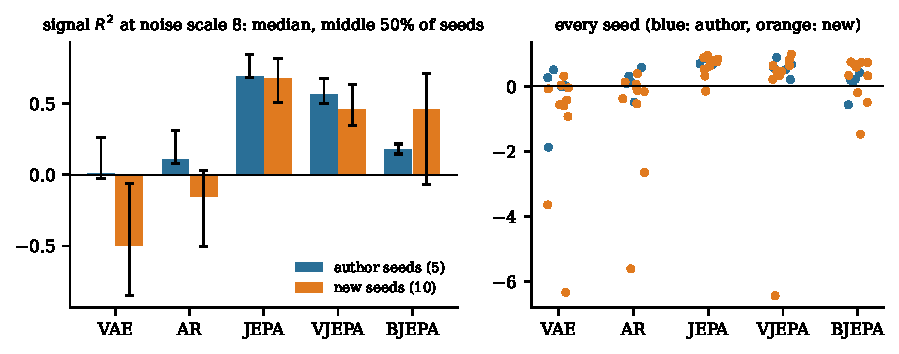
\includegraphics[width=\columnwidth]{figures/huang_reproduction.pdf}
\caption{Variational JEPA reproduction at noise scale 8. Left: median and interquartile range. Right: every seed. One new
seed breaks four of the five models; only deterministic JEPA stays above $-0.2$.}
\label{fig:huang}
\end{figure}

% ------------------------------------------------------------------------------------------------
\section{Final run: further baselines and ablations}
\label{sec:final}
\paragraph{More baselines.} Averaged over the 7 subsets, frozen concatenation has the best NLL (1.380 vs.\ 1.422 for PoE)
and the best calibration error (0.031). MoNIG ranks errors best (Spearman 0.20 vs.\ $-$0.02 for frozen PoE) but is the
worst calibrated (calibration error 0.084) and covers only 0.70 of clips when the text is noise. S-JEPA behaves like V-JEPA
(frozen MAE 0.765 vs.\ 0.770). The ordering of Table~\ref{tab:main} is unchanged.

\paragraph{Corruption, all fusion rules (Noisy TV A/C).} With the text replaced by noise, the fused $\sigma$ changes by a
factor of 0.96--1.00 for every fusion rule while the MAE rises by a factor of 1.09--1.17. Coverage drops to 0.81--0.86
(MoNIG 0.70). Flagging corrupted clips by $\sigma$ is at or below chance for every rule (AUROC 0.22--0.53 for text noise);
disagreement detects swaps only weakly (0.56--0.59).

\paragraph{Calibration decoders.} Per-pattern conformal quantiles (D3m, as in MCCF~\cite{mccf2026}) shrink the worst
per-subset coverage gap from 0.056 to 0.028 for PoE and from 0.124 to 0.029 for MoNIG, so declared missingness is solved
by calibration. No decoder brings silent noise back to 0.90 (best 0.878), because none of them sees that the input is broken.

\paragraph{Ablations of candidate fixes.} Each targets one weakness found above (3 seeds, frozen experts, PoE):
\begin{itemize}
\item \emph{Variational target} (the EMA target is the text expert's Gaussian, not a point): corruption-flag AUROC by
  $\sigma$ rises from \worst{0.38} (V-JEPA) to \best{0.71}; adding a masking ensemble at test time gives 0.74. The
  size of $\sigma$ still barely moves ($\times$1.03), so it ranks corrupted clips correctly without widening their ranges.
\item \emph{Predictor ensemble}, robust PoE and disagreement-aware PoE: identical to PoE on clean and missing inputs
  (NLL 1.422); they only act under conflict, and the predictor ensemble does not detect corruption (AUROC 0.33).
\item \emph{Cross-examined fusion} (CXF: a frozen auditor's joint belief decides which experts to trust). On MOSEI, with an
  alignment auditor, it gives the lowest frozen error under one corrupted sensor (MAE 0.756 vs.\ 0.775) and finds corrupted
  text 92\% of the time, but misses corrupted audio and video. On MS-COCO~\cite{lin2014coco} (image + two captions, object
  count regression) it is the clearest win of the study: MAE 0.570$\rightarrow$0.524 and NLL 1.213$\rightarrow$1.055
  (fine-tuned), and it flags the corrupted sensor with AUROC 0.75--0.95 where $\sigma$ scores 0.10--0.52.
\end{itemize}

\paragraph{Screening 30 techniques.} To search more widely, we screened about 30 techniques (60 variants) from
neighbouring fields on a fast synthetic noisy-TV bench with Gaussian experts: robust statistics (median, Huber,
Student-$t$, trimmed PoE), sensor fault detection (leave-one-out $\chi^2$ gating, RAIM-style exclusion, a Box--Tiao
contamination model, covariance intersection), out-of-distribution detection (input and feature density~\cite{mukhoti2023ddu},
$k$-NN, isolation forest, random network distillation~\cite{burda2019rnd}, a spectral-flatness test from voice activity detection),
cross-modal consistency (ridge predictability, CLIP-style agreement), and self-supervised training (corruption-augmented
experts, an ELECTRA-style~\cite{clark2020electra} ``which modality was replaced?'' classifier). Held-out corruptions that no technique
generated (gain fault, dead sensor, half-clip noise, two bad inputs, a swap from the same speaker) test generalisation, and the
ranking was confirmed on five fresh seeds. Prediction-level robust rules barely help (their only evidence is the experts'
disagreement); input-level detectors flag noise-like faults almost perfectly; the replaced-modality classifier is the only one
that also catches swaps; combined with corruption-augmented experts it matches dropping the true culprit. No technique detects
a swap from the same speaker. On real MOSEI with frozen models, the replaced-modality detector flags held-out corruptions with
AUROC 0.82 and names the right modality 73\% of the time, while $\sigma$ scores 0.43--0.59. It improves NLL only modestly
(6/9 runs), because PoE already tolerates most single-modality corruption on MOSEI; it helps clearly for a dead sensor
(MAE 0.814$\rightarrow$0.761). The replaced-modality idea itself is known (odd-one-out learning~\cite{yang2021oddoneout},
self-supervised corruption prediction~\cite{prime2026}); what our study adds is the uncertainty-centred evaluation.

% ------------------------------------------------------------------------------------------------
\section{Discussion}
\paragraph{What the uncertainty knows.} PoE over Gaussian experts handles \emph{declared} absence well: the tracking
ratio is close to 1 and conformal calibration restores coverage. It fails on \emph{silent} corruption because each expert's
$\sigma$ is computed from that expert's own (corrupted) input. An expert cannot tell from inside that its sensor is broken,
so a confident-but-wrong expert keeps its weight. The information needed to notice, namely that the other modalities
disagree with it, exists in the frozen experts (swap AUROC up to 0.87) but is not used by PoE. Fine-tuning then removes it.

\paragraph{What the objective learns.} Self-predictive targets keep whatever is predictable, including a shared nuisance.
Variational prediction does not change this, and in the single-stream reproduction it is less stable than deterministic
prediction.

\paragraph{Threats to validity.} (i)~One dataset and one label; MOSEI is text-dominated (fine-tuned MAE 0.56 with all modalities vs.\ about
0.81 without text), so audio and video experts are weak. (ii)~Three seeds; the Huang reproduction shows that rare failures need
more. (iii)~In the first run the EMA target encoder kept dropout active during pretraining; the final run fixes this and
reproduces the main results, but changes the noise-modality weights. (vi)~The 30-technique screen uses synthetic data,
which overstated how much one corrupted input hurts compared with MOSEI.
(iv)~Calibration data pools all 46 conditions, 28 of them corruptions, which widens ranges on clean data. (v)~Features are
precomputed; end-to-end encoders may behave differently.

\section{Conclusion and outlook}
Across 144 trained models and 15 reproduction seeds we find that (1)~product-of-experts fusion is the most accurate and
handles missing modalities with well-tracking uncertainty; (2)~the pretraining objective matters only for frozen experts;
(3)~learned Gaussian uncertainty is blind to silently corrupted or swapped inputs; and (4)~self-predictive objectives,
variational or not, absorb a distractor shared across modalities. The final run and ablations add that (5)~a
variational target and cross-examination of the experts are the only changes that make the system notice corruption,
and on a second dataset cross-examination also improves accuracy. The released code adds S-JEPA~\cite{giakoumoglou2026sjepa}, MoNIG~\cite{ma2021monig}, concatenation and
late-fusion baselines, per-pattern conformal calibration, and novel variants (variational target, predictor ensembles,
robust and disagreement-aware PoE). Its runs extend this comparison. Part~II will target the central gap: making each
expert's weight depend on what the \emph{other} modalities say about it, not only on what it says about itself.

{\small
\bibliographystyle{unsrtnat}
\bibliography{refs}
}
\end{document}
